\documentclass[fleqn]{article}
\usepackage{cmap}
\usepackage[left=1in, right=1in, top=1in, bottom=1in]{geometry}
\usepackage{mathexam}
\usepackage{mathtext} 				% русские буквы в фомулах
\usepackage[T2A]{fontenc}			% кодировка
\usepackage[utf8]{inputenc}			% кодировка исходного текста
\usepackage[english,russian]{babel}	% локализация и переносы
\usepackage{enumerate}
%%% Дополнительная работа с математикой
\usepackage{amsmath,amsfonts,amssymb,amsthm,mathtools,amsthm} % AMS
\usepackage{icomma} % "Умная" запятая: $0,2$ --- число, $0, 2$ --- перечисление
\usepackage{graphicx}
%% Шрифты
\usepackage{euscript}	 % Шрифт Евклид
\usepackage{mathrsfs} % Красивый матшрифт
\usepackage{mathtools}
\ExamClass{SE Academic University}
\ExamName{Homework 11}
\ExamHead{\today}

%% Шрифты
\usepackage{euscript}	 % Шрифт Евклид
\usepackage{mathrsfs} % Красивый матшрифт

%Листинг кода
%\usepackage{listings}
\usepackage{listingsutf8}
\usepackage{color}

\renewcommand{\qedsymbol}{$\blacksquare$}
%Для листинга кода
\definecolor{mygreen}{rgb}{0,0.6,0}
\definecolor{mygray}{rgb}{0.5,0.5,0.5}
\definecolor{mymauve}{rgb}{0.63,0.082,0.082}


\lstset{
	inputencoding=utf8,
	%
	backgroundcolor=\color{white},   % choose the background color; you must add \usepackage{color} or \usepackage{xcolor}
	basicstyle=\footnotesize,        % the size of the fonts that are used for the code
	breakatwhitespace=false,         % sets if automatic breaks should only happen at whitespace
	breaklines=true,                 % sets automatic line breaking
	captionpos=b,                    % sets the caption-position to bottom
	commentstyle=\color{black},    % comment style
	deletekeywords={...},            % if you want to delete keywords from the given language
	escapeinside={\%*}{*)},          % if you want to add LaTeX within your code
	extendedchars=\true,              % lets you use non-ASCII characters; for 8-bits encodings only, does not work with UTF-8
	frame=false,                    % adds a frame around the code
	keepspaces=true,                 % keeps spaces in text, useful for keeping indentation of code (possibly needs columns=flexible)
	keywordstyle=\color{blue},       % keyword style
	morekeywords={*,...},            % if you want to add more keywords to the set
	numbers=left,                    % where to put the line-numbers; possible values are (none, left, right)
	numbersep=5pt,                   % how far the line-numbers are from the code
	numberstyle=\tiny\color{black}, % the style that is used for the line-numbers
	rulecolor=\color{white},         % if not set, the frame-color may be changed on line-breaks within not-black text (e.g. comments (green here))
	showspaces=false,                % show spaces everywhere adding particular underscores; it overrides 'showstringspaces'
	showstringspaces=false,          % underline spaces within strings only
	showtabs=false,                  % show tabs within strings adding particular underscores
	stepnumber=1,                    % the step between two line-numbers. If it's 1, each line will be numbered
	stringstyle=\color{black},     % string literal style
	tabsize=4                  % sets default tabsize to 2 spaces
	% show the filename of files included with \lstinputlisting; also try caption instead of title
}   

\usepackage{hyperref}

\let\ds\displaystyle

\begin{document}
	%\section*{Декартовы деревья}
\begin{enumerate}
	\item Пусть \textbf{splay}-дерево поддерживает множество $S$. Каждый элемент $x_i \in S$ был запрошен $p_im$ раз, где $m$ — общее число запросов. 
	Гарантируется, что $0 < pi \leqslant 1$ и $\sum_ip_i = 1$. Докажите, что \textbf{splay}-дерево обрабатывает все запросы за время $O(m\cdot \left[1 + \sum_ip_i\cdot \log \frac{1}{p_i} \right])$.

	\textbf{Решение.} 
	
	Введем весовую функцию $\omega(x_i) = p_i$. Тогда $s(x)$ - вес поддерева с корнем в $x$. А $r(x) = \log_2 s(x)$ - ранг вершины $x$.
	
	Обозначим $root$ - корень дерева. Из теории известно, что амортизированное время $splay$ не превышает $1 + 3(r(root) - r(x)$.
	
	Посчитаем тогда амортизированное время для всех $m$ запросов. 
	
	$$m + 3mr(root) - 3\sum\limits_{i = 1}^{n} p_i\cdot m\cdot r(x_i) \leqslant m + 3mr(root) - 3\sum\limits_{i = 1}^{n} p_i\cdot m\cdot \log_2 \omega(x_i)$$
	
	$$m(1 + 3 r(root) - 3 \sum\limits_{i = 1}^{n} p_i\cdot \log_2 p_i) = 
	m(1 + 3 r(root) + 3 \sum\limits_{i = 1}^{n} p_i\cdot \log_2 \frac{1}{p_i})$$
	
	Учитывая, что $root$ - корень, и $s(root) = 1$, значит, $r(root) = \log_2 s(root) = 0$, а сумму $\sum\limits_{i = 1}^{n} p_i\cdot \log_2 \frac{1}{p_i}$ можно ограничить снизу и сверху, и, значит, последнее выражение можно переписать в виде $O(m\cdot \left[1 + \sum_ip_i\cdot \log \frac{1}{p_i} \right])$
	
	\item Придумайте структуру данных, поддерживающую упорядоченный список S целых чисел, которая
	умеет отвечать на запросы:
	\begin{itemize}
		\item $insert(x)$ — вставить $x$ в $S$, если его там не было.
		\item $delete(x)$ — удалить $x$ из $S$, если он там был.
		\item $S[k]$ — вернуть $k$-ый по порядку элемент из $S$.
		\item $\max(l, r)$ — найти $\max_{l\leqslant j<k\leqslant r} |S[j] - S[k]|$. Гарантируется $r - l \geqslant 1$.
		\item $\min(l, r)$ — найти $\min_{l\leqslant j<k\leqslant r} |S[j] - S[k]|$. Гарантируется $r - l \geqslant 1$.
	\end{itemize}
	
	Каждый запрос должен обрабатываться за $O(\log |S|)$.
	
	\item Пусть приоритеты случайны, а ключи все разные. Найдите матожидание количества листьев в
	Декартовом дереве из $n$ вершин.
	
	\textbf{Решение.}
	
	Идея. Выпишем рекуррентное соотношение для матожидания и решим его.
	Заметим, что любой ключ может попасть в корень с равной вероятностью, которая равна 
	$\frac{1}{n}$. После этого матожидание количества листьев равна сумме матожиданий количества листьев в правом и левом поддеревьях корня. Просуммируем по всем $i$, получим следующее соотношение:
	
	$$E_n = \sum\limits_{i = 1}^{n} (E_{i - 1} + E_{n - i}) \frac{1}{n}$$
	
	Заметим, что в этой сумме мы все слагаемые $E_i$ посчитали ровно по два раза. Тогда:
	
	$$E_n = \frac{2}{n} \sum\limits_{i = 0}^{n - 1} E_i$$
	
	$$\frac{n}{2} E_n = \sum\limits_{i = 0}^{n - 1} E_i$$
	
	Запишем то же выражение для $n - 1$:
	
	$$\frac{n - 1}{2}E_{n - 1} = \sum\limits_{i = 0}^{n - 2} E_i$$

	Вычтем его из выражения выше для $E_n$. Получим соотношение для $E_{n - 1}$
	
	$$E_{n - 1} = \frac{n}{2} E_{n} - \frac{n - 1}{2} E_{n - 1}$$
	
	Упростим его
	
	$$\frac{n}{2} E_n = \frac{n + 1}{2}E_{n - 1}$$
	
	$$E_n = \frac{n + 1}{n} E_{n - 1}$$
	
	Последнее выражение можно последовательно раскрутить, сократив одинаковые выражения в числителе и знаменателе, пока не получим тривиальное значение $E_2 = 1$.
	
	$$E_n = \frac{n + 1}{n} \frac{n}{n - 1} \frac{n - 1}{n - 2} \cdots \frac{4}{3} E_2 = \frac{n + 1}{3} \cdot 1 = \frac{n + 1}{3}$$
	
	Таким образом, ответом является значение $\dfrac{n + 1}{3}$
	
	\item Пусть приоритеты случайны, а ключи все разные. Обозначим за $x_k$ вершину Декартова дерева,	содержащую $k$-ый по порядку ключ. Всего в дереве $n$ вершин.
	\begin{itemize}
		\item Пусть $1 \leqslant i \leqslant j \leqslant k \leqslant n$. Найдите вероятность того, что $x_j$ — общий предок $x_i$ и $x_k$.
		\item Пусть $1 \leqslant i \leqslant k \leqslant n$. Найдите матожидание длины пути между $x_i$ и $x_k$.
	\end{itemize}
	
	
	
	\item Т.к. обычно приоритеты в Декартовом дереве случайны, то их хранение выглядит избыточным.
	Попробуем их не хранить, а во время операции merge будем делать следующее: если в дереве
	$A$ $n_A$ элементов, а в дереве $B$ $n_B$ элементов, то с вероятностью 
	$\frac{n_A}{n_A + n_B}$ в качестве корня будет выбран корень дерева $A$, а с вероятностью 
	$\frac{n_B}{n_A + n_b}$ в качестве корня будет выбран корень дерева $B$ (далее слияние 
	происходит аналогично слиянию в Декартовом дереве).
	
	Оцените высоту такого дерева поиска.
	
	\textbf{Решение.}
	
	
	
	\item Придумайте структуру данных, которая поддерживает следующие операции:
	
	\begin{itemize}
		\item Вставка символа на позицию $i$;
		\item Удаление символов с позиций $[l, r)$;
		\item Копирование подстроки $[l, r)$ в позицию $i$ (пример: $l = 1, r = 4, i = 5 : abcdefg \leftarrow abcdebcdfg$
	\end{itemize}
	
	Все операции должны выполнятся за логарифмическое время от текущей длины текста.
	
	\textbf{Решение.}
	
	
\end{enumerate}

\section*{Дополнительные задачи}
\begin{enumerate}
	\item Придумайте аналог Декартова дерева со случайными приоритетами для хранения точек на плоскости с операциями $splitX, mergeX, splitY, mergeY$. Все операции должны работать за $o(n)$.
\end{enumerate}


	%\section*{RMQ и LCA}
\begin{enumerate}
	\item Дано дерево из одной вершины. Требуется уметь отвечать $online$ за $O(\log n)$ на
	запрос: подвесить новую вершину $u$ к вершине дерева $v$ и вернуть диаметр дерева. Диаметр
	дерева — длина самого длинного простого пути в дереве. 
	
	\textbf{Решение.} 
	
	Заметим, что самый длинный путь в дереве - путь между какими-либо двумя листьями (пусть это 
	не так, и существует путь, хотя бы одна вершина которого - не лист. Но тогда можно 
	продолжить этот путь минимум на 1 вершину. Значит путь не максимальный. Противоречие.)
	
	Заметим, что при добавлении вершины мы всегда добавляем лист. 
	
	Ещё одно \textbf{ утверждение}: \textit{в дереве не может быть два пути максимальной длины 
	(обозначим макс. длину пути $M$), которые не пересекаются.} (Если они есть, то можно 
	построить путь большей длины: выберем самую верхнюю вершину первого пути, и самую верхнюю 
	вершину второго пути. Они не могут совпадать, и между ними есть хотя бы одно ребро. Каждая 
	из этих вершин разбивает соответствующий путь на две части. Выберем из этих частей бОльшие, 
	длина каждой части, минимум, $M / 2$. А значит, можно построить путь длиной не менее $M + 
	1$, что противоречит о максимальности выбранных путей.)
	
	\textbf{Следствие.} Все пути максимальной длины в дереве пересекаются. 
	
	Заметим, что длина максимального пути может измениться не более чем на единицу(т.к. 
	добавляется только 1 вершина и одно ребро), и изменится она только лишь в том случае, когда 
	вершина добавляется к одному из концов какого-либо пути максимальной длины.
	
	Теперь заметим, что поддерживая концевые вершины одного из кратчайших путей, можно понять, 
	изменяет ли добавление вершины длину пути наибольшей длины. Для этого воспользуемся $LCA$, 
	и будем хранить на каком расстоянии от корня находится каждая вершина. Так же будем хранить 
	две вершины(обозначим $v_b, v_e$), которые образуют путь максимальной длины в дереве 
	(сначала она равны одной заданной вершине). При добавлении вершины $u$ будем искать, при 
	помощи $LCA$ ближайшего общего предка для пар вершин $u$, $v_b$, и так же $u$, $v_e$. И, 
	зная расстояния от корня для всех вершин можно будет рассчитать длину путей из $u$ в $v_b$ 
	и из $u$ в $v_e$. Если длина какого либо из них превзойдет длину пути $v_b \to v_e$, то 
	заменим соответствующую вершину на $u$ и вернем полученное значение длины максимального 
	пути.
	
	\textbf{Оценка сложности.} 
	
	Использование $LCA$ имеет сложность $O(\log n)$. Операции вычисления длин двух путей и их 
	сравнение с длинами старых путей, очевидно, константные.
	
	\textbf{Корректность.} 
	
	Разбором случаев пересечений пары двух путей максимальной длины можно получить, что если
	добавленное значение увеличивает один из путей макс. длины, то можно увеличить и старый путь макс.
	длины, заменив одну из его граничных вершин. 
	
	\item Дан ориентированный граф, в котором исходящая степень каждой вершины равна единице.
	Запросы $online$: из вершины $v$ сделать $k$ шагов вперед.
	\begin{itemize}
		\item Предподсчет: $O(n \log k\max)$, время на запрос: $O(\log k)$.
		\item Предподсчет: $O(n \log n)$, время на запрос: $O(\log \min(k, n))$.
	\end{itemize}
	
	\textbf{Решение.}
	
	\begin{itemize}
		\item Предподсчет: $O(n \log k\max)$, время на запрос: $O(\log k)$.
		
		Сделаем скип-лист через каждые $1, 2, 4, 8, 16, ..., k_max$ элементов, тогда сможем за $O(\log k)$ отвечать на запрос.
		\item Предподсчет: $O(n \log n)$, время на запрос: $O(\log \min(k, n))$.
		
		В этом случае нужно воспользоваться структурой графа. В графе обязан быть хотя бы один 
		цикл, поэтому при больших $k$ движение вперед рано или поздно зациклится. Идея в том, 
		чтобы дойти до вершины из цикла, затем убрать лишние циклы из $k$, и пройти оставшееся 
		количество шагов по скиплисту.
		
		На первом шаге алгоритма найдем все циклы в графе с помощью какого-либо обхода, и для 
		каждой вершины сохраним 0, если она не входит ни в какой цикл, и значение длины цикла, 
		если входит. Так же построим скип-лист через каждые $1, 2, 4, 8, 16, ..., n$ вершин. 
		При запросе так же будем двигаться по скип листу, до тех пор, пока не сделаем все шаги, 
		либо пока не попадем в вершину которая лежит в каком-либо цикле. После этого удалим из 
		оставшегося числа шагов полные циклы, и выполним те шаги, что остались. 
		
		\textbf{Оценка сложности.} 
		
		Т.к. теперь скип-лист строится до шага длины $n$, то преподчсчет займет $O(n \log n)$. 
		А т.к. добраться до цикла можно в худшем случае за $O(\log n )$ шагов, а выбросить 
		циклы из значения $k$ займет $O(1)$, то время на запрос составит $O(\log \min(k,n))$. 
	\end{itemize}
	
	\item Дан массив чисел длины $n$. За $O(\log n)$ в $online$ обрабатывать запросы:
	\begin{itemize}
		\item посчитать сумму кубов чисел на отрезке $[L, R]$
		\item прибавить $x$ ко всем числам на отрезке $[L, R]$
		\item получить значение $i$-го числа
	\end{itemize}
	
	\textbf{Решение.}
	
	Воспользуемся $RMQ$, в узле будем хранить значение суммы, суммы квадратов и кубов.
	
	Почему нужно именно это? Рассмотрим сумму кубов на отрезке $[L, R]$:
	
	$$\sum (a_i + x)^3 = \sum (a_i^3 + 3a_i^2x + 3a_ix^2 + x^3) = \sum (a_i^3) + 3x\sum(a_i^2) + 3x^2\sum a_i + (R-L)x^3$$
	
	$$\sum (a_i + x)^2 = \sum (a_i^2 + 2a_ix + x^2) = \sum (a_i^2) + 2x\sum(a_i) + (R-L)x^2$$
	
	$$\sum (a_i + x) = \sum(a_i) + (R-L)x$$
	
	То есть имея эти три значения, можно пересчитывать сумму кубов на отрезке, не пересчитывая 
	её на подотрезках, выполняя второй запрос за $O(\log n)$. 
	
	Заметим теперь, что на подотрезках мы не вычислили сумму кубов, квадратов и значений. Для 
	этого в каждом узле будем хранить два отложенных вычисления - сколько нужно добавить в 
	левый подотрезок и сколько нужно добавить в правый подотрезок. И при выполнении запросов эти отложенные вычисления нужно проталкивать ниже. 
	
	\textbf{Оценка сложности.} 
	
	Достаточно заметить, что пересчет сумм кубов, квадратов и самих значений занимает $O(1)$, значит сложность запроса составит сложность работы с $RMQ$, то есть - $O(\log n)$.
	
	\item Дана скобочная последовательность из круглых скобок длины $n$. Запросы: является ли 
	отрезок $[L, R]$ правильной скобочной последовательностью; изменить $i$-ю скобку. $O(\log 
	n)$, $online$.
	
	\textbf{Решение.}
	
	Введем понятие баланса скобочной последовательности - разность между количеством 
	открывающим и закрывающих скобок. Значение баланса можно вычислять на префиксе скобочной 
	последовательности. Пусть $a_i$ - значение баланса на префиксе длины $i$. Тогда для того, 
	чтобы отрезок $[L, R]$ образовывал правильную скобочную последовательность необходимо, 
	чтобы $a_L$ было равно $a_R$ (то есть количество открывающих и закрывающих скобок совпало), 
	и так же, ни на каком префиксе $[L:i]$ не нарушился баланс скобок. То есть $a_L \leqslant 
	\min_{i\in[L, R]} a_i$.
	
	При запросе изменения скобки на $j$ позиции нужно пересчитать балансы на суффиксе 
	последовательности после элемента $j$.
	
	Для решения задачи можно воспользоваться $RMQ$, для массива $a_i$ - балансов скобочной 
	последовательности.
	
	\item Попробуем модифицировать идею $\mathbf{SparseTable}$ так, чтобы она работала для 
	произвольных ассоциативных функций: предложите способ выделить $O(n \log n)$ отрезков в 
	массиве размера $n$ так, что любой отрезок $[L, R]$ можно было представить в виде 
	объединения $O(1)$ непересекающихся выделенных отрезков. Заметим, что дерево отрезков 
	выделяет $O(n)$ отрезков, и любой отрезок представляется как объединение $O(log n)$ из них.
	
	\textbf{Решение.}
	
	Сохраним в таблице только значения для отрезков вида $[i, n/2), [n/2, i)$, где $i\in 0, 1, 
	2,..., n - 1$. Аналогично сохраним значения для отрезков вида $[i, n/4), [n/4, i)$, где 
	$i\in 0, 1, 2,..., n/2 - 1$. и $[i, 3n/4), [3n/4, i)$ где $i\in n/2, n/2 + 1,..., n - 1$.
	и т.д. На каждом шаге вычисляем значения для $O(n)$ отрезков. Всего шагов - $O(\log n)$.
	
	Теперь заметим, что при таком разбиении можно любой отрезок разбить на два других, для 
	которых значения уже вычислены. Рассмотрим отрезок $[L, R]$, найдем i, k, такие 
	$\min\limits_{i > 0} : L\leqslant k*n/2^i \leqslant R$
	
	Найдя такие $i, k$ мы сможем разбить отрезок $[L,R] = [L, k*n/2^i) \cup [k*n/2^i, R]$. 
	
	\item Дан массив из $n$ элементов. Запросы: $k$-е по порядку среди различных чисел на отрезке $[L, R]$.
	\begin{itemize}
		\item $offline$ за $O(\log^3 n)$.
		\item $online$ за $O(\log^3 n)$.
	\end{itemize}
	
	\item Придумайте структуру данных, которая поддерживает следующие операции:
	
	\begin{itemize}
		\item Вставка символа на позицию $i$;
		\item Удаление символов с позиций $[l, r)$;
		\item Копирование подстроки $[l, r)$ в позицию $i$ (пример: $l = 1, r = 4, i = 5 : abcdefg \leftarrow abcdebcdfg$
	\end{itemize}
	
	Все операции должны выполнятся за логарифмическое время от текущей длины текста.
		
	!! Обратите внимание, т.к. теперь распределение вершин в левом и правом поддереве не 
	независимы, свести оценку глубины напрямую к qsort — не получится.
		
\end{enumerate}



	%\section*{Деревья и пути}
\begin{enumerate}
	\item Назовем ребро дерева тяжелым, если размер поддерева, его нижнего конца больше либо равен 
	половине размера поддерева его верхнего конца. Покроем дерево путями следующим способом: из 
	каждой вершины, в которую входит тяжелое ребро будем идти вверх, пока не дойдем до корня, 
	или пока не пройдем по легкому ребру. Такое покрытие называется 
	\textbf{«Heavy-Light-Decomposition»}. Докажите, что путь из любой вершины в корень пересекает 
	не более чем $\log n$ путей из покрытия, где $n$ — количество вершин.
	
	\textbf{Решение.} 
	
	Рассмотрим путь от произвольной вершины до корня. Будем двигаться по нему 
	в обратном направлении - от корня к вершине. При переходе к следующей вершине возможны два 
	случая: прошли по тяжелому ребру $\Rightarrow$ остались в прежнем пути, либо прошли по 
	легкому ребру, значит начался другой путь. Заметим, что когда проходим по легкому ребру, то 
	размер поддерева, в котором находится вершина уменьшился как минимум в 2 раза (иначе это 
	ребро было бы тяжелым). Таким образом, смена пути покрытия в пути от корня к произвольной 
	вершине влечет за собой уменьшение не менее чем в 2 раза размер поддерева, значит и путей 
	покрытия, которые пересеклись с рассмотренным путем не более чем $\log_2 n$.
	
	\item Дано дерево, у каждой вершины есть вес. Запросы: 
	изменить вес вершины; 
	найти максимум на пути из $u$ в $v$. $\langle O(n \log n)$, $O(\log^2 n) \rangle$. 
	
	Hint: предыдущая задача.
	
	\item Даны подвешенное дерево и его Эйлеров обход. Придумайте, как за $O(\log n)$ обновить 
	Эйлеров	обход при переподвешивании дерева за другую вершину (для разных вариантов обхода).
	
	\item Пусть есть много неподвешенных деревьев. Запросы \textit{online}:
	\begin{itemize}
		\item соединить ребром вершины $v$ и $u$ разных деревьев,
		\item удалить ребро между вершинами $v$ и $u$,
		\item проверить, в одной ли компоненте лежат вершины $u$ и $v$.
	\end{itemize}
	
	$O(n)$ на предобработку, $O(\log n)$ на запрос ($n$ — суммарный размер деревьев).
	
	\textbf{Решение.} 
	
	Заметим, что для подвешенных деревьев мы умеем решать эту задачу. В предыдущей задаче мы 
	научились обновлять за $O(\log n)$ Эйлеров обход дерева при переподвешивании за другую 
	вершину.
	
	Предобработка: подвесим все имеющиеся деревья за произвольную вершину, найдем для них 
	Эйлеровы обходы  с построим Декартово дерево по неявному ключу. 
	
	Ответы на запросы:
	
	\textit{соединить ребром вершины $v$ и $u$ разных деревьев}. Переподвесить дерево, в 
	котором находится вершина $u$ за эту вершину. Соединить полученное подвешенное дерево с 
	вершиной $v$.
	
	\textit{удалить ребро между вершинами $v$ и $u$}. Переподвесим дерево за $u$. Теперь $v$ 
	является корнем своего поддерева, задача сведена к уже решенной.
	
	\textit{проверить, в одной ли компоненте лежат вершины $u$ и $v$.} В любой момент времени 
	все деревья подвешены. Такая задача уже решена.
	
	
	
	\item Дано дерево из n вершин, по которому бегают муравьи. Вам поступает $m$
	запросов вида $a, b$, что означает, что очередной муравей пробежал из вершины $a$ в вершину 
	$b$.
	
	\begin{enumerate}
		\item Выведите, сколько раз муравьи пробежали через каждое из ребер за $O(n + m)$.
		\item А теперь вам онлайн поступают вопросы про каждое из ребер (эти запросы могут поступить в любой момент, в том числе до окончания муравьиных пробегов). Обработайте каждый из двух типов запросов за $log_2 n$ с предподсчетом за $O(n \log n)$.
	\end{enumerate}
\end{enumerate}



	%\section*{Хеширование}
\begin{enumerate}
	\item Семейство хэш-функций $\mathcal{H} = \{h : X \rightarrow Y \}$ называется универсальным, если:
	
	\begin{equation*}
	\forall x_1, x_2 \in X, x_1 \neq x_2 : \underset{h \in \mathcal{H}}{\mathbf{Pr}} \left[h(x_1) = h(x_2)\right] 
	\leqslant \frac{1}{|Y|}
	\end{equation*}
	
	Семейство хэш-функций $\mathcal{H} = \{h : X \rightarrow Y \}$ называется $k$-независимым, если для любых 
	различных $x_1, x_2, \cdots , x_k \in X$, для любых, возможно совпадающих, выполняется: $y_1, y_2, \cdots, 
	y_k \in Y$
	
	\begin{equation*}
	 \underset{h \in \mathcal{H}}{\mathbf{Pr}} \left[\bigwedge\limits_{i = 1}^{k} h(x_i) = y_i\right] = 
	 \frac{1}{|Y|^k}
	\end{equation*}
		
	\begin{enumerate}
		\item Докажите, что из любое 2-независимое семейство хэш-функций является универсальным.
		\item Докажите, что любое $k + 1$-независимое семейство хэш-функций является $k$-независимым.
	\end{enumerate}
	
	
	\item В вашем распоряжении есть пара 2-независимых семейств хеш-функций $\mathcal{A} = \{f : A \rightarrow 
	F_2^n \}$ и $\mathcal{B} = \{g : B \rightarrow F_2^n \}$. Постройте (и докажите, что построено правильно) 
	универсальное семейство хеш-функций, которое:
	\begin{enumerate}
		\item будет отправлять пары типа $(A, B)$ в $F_2^n$,
		\item будет отправлять мультимножества из элементов типа $A$ в $F_2^n$,
		\item будет отправлять множества из элементов типа $A$ в $F$,
		\item будет отправлять списки из элементов типа $A$ в $F_2^n$.
	\end{enumerate}
	
	\item Используя функцию из задания 10 с практики, постройте семейство 2-независимых хэш-функций $\mathcal{H} 
	= \{h_i: \mathbb{F}^n_2 \rightarrow \mathbb{F}^n_2\}_i$ Докажите, что семейство является 2-независимым.
		
	\item[4*.] Пусть дана хэш-таблица размера $n$ с хэш-функцией $h : K \rightarrow [n]$. На вход поступает $n$ 
	ключей. Будем предполагать, что хэш-функция отправляет каждый ключ в каждую ячейку независимо с равной 
	вероятностью. Коллизии разрешаются с помощью односвязных списков, цепочек. Посчитаем максимальную длину 
	цепочки.
	
	\begin{enumerate}
		\item Зафиксируем хэш-значение $x$. Доказать, что вероятность, что $k$ ключей будут иметь хэш $x$ 
		составляет
		
		\begin{equation*}
			Q_k = \binom{n}{k}\cdot \left( \frac{1}{n} \right)^k \cdot \left(1 - \frac{1}{n} \right)^{n-k}
		\end{equation*}
		
		\textbf{Решение.} Раз уж испытания независимы, то можно их интерпретировать как схему Бернулли. Первый 
		множитель, это количество способов выбрать $k$ элементов из $n$, значение хеша от которых равно $x$. 
		Второй множитель - вероятность, что эти $k$ элементов перейдут в $x$. Последний множитель - вероятность, 
		что остальные $n - k$ элементов перейдут во что-то другое, но не $x$.
		
		\item Пусть $P_k$ – вероятность максимальной цепочки иметь длину $k$. Доказать, что $P_k \leqslant n 
		\cdot Q_k$.
		
		\item Вывести из Стрилинга, что $Q_k \le \left(\dfrac{e}{k}\right)^k$
		\item Показать, что для некоторого $c \ge 1$ верно $Q_k \leqslant c \cdot \dfrac{\log n}{\log \log n}$.
	\end{enumerate}
	
	\item[7.] Пусть мы можем потратить не более 100 байт памяти на предподсчет. Нужно научится по 64-битному 
	числу вида $2^k$ восстанавливать $k$ за $O(1)$ арифметических операций и единственное
	чтение одного байта из предподсчитанных данных. Напишите псевдокод предподсчета и ответа на 
	запрос.
	
	\textbf{Решение.}
	
	Для решения этой задачи нам потребуется циклическая группа, элемент-генератор которой равен $2$, а количество 
	элементов превосходит 64. Для этих целей нам подойдут 2 группы $\mathbb{Z}_{67}$ и $\mathbb{Z}_{83}$ по 
	умножению. Выберем $\mathbb{Z}_{67}$. Тогда каждая степень двойки перейдёт в свой элемент группы и мы сможем 
	числа $2^0, 2^1, 2^2, ..., 2^{63}$ однозначным образом хешировать (Одного байта, чтобы записать степень, не превосходящую 64 нам вполне достаточно.). То есть преподсчет будет следующий:
	\begin{lstlisting}
	byte buf[100]
	for k = 0..63:
		buf[2**k % 67] = k
	\end{lstlisting}
	А для определения степени $k$ для значения $p$ можно воспользоваться:
	\begin{lstlisting}
	k = buf[p % 67]
	\end{lstlisting}
	
	\item[8.] Вам даны два корневых дерева, большое $T$ и маленькое $t$. Требуется найти такую вершину $x$
	дерева $T$, что поддерево, индуцированное вершиной $x$, и $t$ изоморфны.
	
	Решайте в предположении, что у вас есть хорошие хеш-функции для списков.
	
	\begin{enumerate}
		\item При проверке на изоморфизм порядок детей важен,
		
		\textbf{Решение.} В каждой вершине дерева $T$ будем хранить значение хеша, которое соответствует его 
		поддереву. Чтобы вычислить хеш, необходимо: во все листья записать значение хеша равный $0$. Хеш вершине 
		равен хешу списка хешей потомков(список содержит хеши в порядке потомков). Осталось аналогичным образом 
		вычислить хеш для дерева $t$ и проверить, встречается ли это значение в хешах для какой-либо вершины 
		дерева $T$. 
		
		\item При проверке на изоморфизм порядок детей не важен.
		
		\textbf{Решение.} Аналогично предыдущему пункту, с той лишь разницей, что прежде чем вычислять хеш от 
		списка с хешами потомков, этот список нужно отсортировать, тогда порядок потомков станет не важен. 
	\end{enumerate}
	
	\textbf{Дополнительная задача.}
	
	\item[1.] Придумайте решение последней задачи без использования хеш-функций.
	
	Решение описано в статье:
	
	\url{http://logic.pdmi.ras.ru/~smal/files/smal_jass08.pdf}
	
	\textbf{Задача про фильтр Блума.}
	
	\item[1.] Пусть имеется фильтр Блума длины $m$ с $k$ функциями. Фильтр Блума можно использовать для подсчета количества 
	различных элементов в множестве. Известно, что матожидание количества бит, выставленных фильтром Блума $n(A)$ 
	связанно с количеством различных элементов в множестве $A$ следующей функцией:
	\begin{equation}
		|A| = - \dfrac{m \ln (1-\frac{n(A)}{m})}{k}
	\end{equation}
	Придумайте, как, имея фильтры Блума для множества $A$ и $B$, оценить размер пересечения и размер объединения 
	данных множеств.
	
	\textbf{Решение.} Достаточно вспомнить с практики, что для объединения будет просто дизъюнкция. 
	
	А размер пересечения можно получить из формулы включения-исключения:
	
	$|A \cap B| = |A| + |B| - |A \cup B|$
	
\end{enumerate}



	%\section*{Алгебра}
\begin{enumerate}
	\item Дана матрица $A$ размера $n \times m$. Найти такое представление $A = B \cdot C$, что $B$ имеет размер $n 
	\times k$ и $k$ минимально.
	
	\textbf{Решение.} Искомое разложение можно получить, воспользовавшись
	 \url{https://en.wikipedia.org/wiki/Rank_factorization}.
	 
	 Осталось понять, почему в таком разложении $k$ минимально. Для ранга произведения двух матриц справедливо следующее утверждение (общий факт из линейной алгебры):
	 \begin{equation*}
	 	rank(A) = rank(BC) \leqslant \min(rank(B), rank(C))
	 \end{equation*}
	 
	 Из неравенства видно, что взять $k$ меньше чем ранг невозможно. В нашем разложении $k = rank(A) = rank(B) = 
	 rank(C)$
	
	\item Для заданного $n$ и простого $p$ найти число таких $k \in [0, n]$, что $\binom{n}{k} \mod p = 0$. Можно 
	считать, что все операции по модулю $p$ происходят за $O(1)$. Придумайте алгоритм, который работает за:
	\begin{enumerate}
		\item $O(n)$
		
		\textbf{Решение.} Вспомним формулу:
		\begin{equation*}
		\binom{n}{k} = \frac{n!}{k!(n - k)!}
		\end{equation*}
		
		Заметим, что это значение может быть представлено в виде $\binom{n}{k} = p^m \cdot r$. Где $r$- число, 
		которое не делится на $p$, а $m$ - некоторое неотрицательное число (бин. коэффициент не может быть 
		дробным).
		
		Осталось научиться быстро искать $m$ для разных значений $k$.
		
		Можно воспользоваться следующей динамикой для предподсчета степеней $p$, которые входят в $1!, 2!, .., 
		n!$ и в значения $1,2,3, .., n$. Массив для первой динамики обозначим $d$, для второй $r$.
		\begin{align*}
			&r[1, ..., p - 1] = 0 \\
			&r[i] = 0, i \neq 0 (mod \ p) \\
			&r(i) = r(i / p) + 1, i = 0(mod \ p)
		\end{align*}
		
		И вторая:
		\begin{align*}
		&d[1] = d[2..p-1] = 0 \\
		&d[i] = d[i - 1], i \neq 0 (mod \ p) \\
		&d[i] = d[i - 1] + r[i], i = 0(mod \ p)
		\end{align*}
		
		Теперь, заметим, что $m = d[n] - d[k] - d[n - k]$. Это можно вычислить за $O(1)$, осталось лишь найти количество таких $k$ из интервала $[1, n]$. 
		
		\textbf{Сложность:} $O(n)$ на каждую из динамик $O(n)$ на поиск всех $k$. Итого $O(n)$.
		
		\item $O(loly(\log n))$ (Подсказка: попробуйте представить числа в $p$-ичной системе счисления и 
		упростить $(x + 1)^n$)
		
		Можем воспользоваться теоремой Лукаса \url{https://en.wikipedia.org/wiki/Lucas'_theorem}, тогда
		\begin{equation*}
		\binom{n}{k} = \prod_{i=0}^d\binom{n_i}{k_i}\pmod p,
		\end{equation*}
		Где $n_i, k_i$ - разряды разложения чисел $n,k$ в $p$-ичную систему исчисления. Такие разложения можем 
		найти за $O(\log n)$.
		
		Тогда, чтобы произведение было равно $0$, необходимо, чтобы хотя бы один множитель был равен $0$. Чтобы 
		проверить, множитель равен $0$ достаточно сравнить $n_i$ с $k_i$, и если $k_i > n_i$, то коэффициент 
		равен 0, и ответ на вопрос задачи положительный. А т.к. количество слагаемых не превосходит $O(\log n)$, 
		то и все сравнения мы успеем сделать за $O(\log n)$.
		
	\end{enumerate}
	
	\item На кольцевой стоят $n$ светофоров и хитро перемигиваются. Свет на каждом светофоре зажигается в таком 
	порядке: зелёный-жёлтый-красный, снова зелёный и так по кругу. Все светофоры пронумерованы от $1$ до $n$. Если 
	светофор по номеру $i$ решит поменять свой цвет то следующие, $k_i$ светофоров с шагом $a_i$ тоже поменяют свой 
	цвет.
	
	По начальному состоянию светофоров определите, возможен ли зелёный коридор. Т.е. такая ситуация, когда все 
	светофоры переключены на зелёный. Решить за $O(n^3)$.
	
	\textbf{Решение.}
	
	Для начала скажем, что значения $a_i$ можно взять по модулю $n$, т.к. у нас светофоры стоят в кругу, и 
	наматывать круги большого смысла нет. Так же заметим, что после $lca(a_i, n)$ шагов мы точно начнём ходить по 
	тем же светофорам, а после $3*lca(a_i, n)$ и вовсе делать то же самое. Поэтому, можно считать, что мы то же 
	самое не делаем, и все $k_i$ ограничены $n^2$. 
	
	Теперь заполним матрицу $L_{n\times n}$, где $l_{ij}$ - количество переходов светофора с номером $j$, после 
	того, как светофор $i$ сменил свой цвет. За $O(n^3)$ мы это успеем сделать, т.к. каждую строку мы заполняем 
	не более чем за $O(n^2)$ переходов. 
	
	Очевидно, что порядок включений светофоров не важен. Тогда попытаемся понять, как же определить какого цвета 
	станет светофор с номером $i$ после каких-то переключений светофоров, где светофор номер $1$ переключится 
	$k_1$ раз, второй $k_2$ раз, и т.д. до $k_n$. Тогда цвет светофора номер $j$ определяется его начальным 
	состоянием($state_j$) и переходами, которые были вызваны переключениями других светофоров. Будем считать, что 
	зелёному соответствует $0$, жёлтому $1$, красному $2$.
	\begin{equation*}
		s_j = state_j + \sum\limits_{i = 1}^{n} L[i][j] * k_i = 0
	\end{equation*}
	
	Несложно заметить, что записав такие равенства для всех светофоров мы получим СЛАУ с матрицей $L^T$, вектором 
	неизвестных из $k_i$ и вектором правой части из начальных состояний. Попытаемся её решить (по простому модулю 
	3), Если получится, то последовательность переключений будет решением, если решения нет, то и 
	последовательности тоже нет.
	 
	\item У Винни-Пуха есть бесконечные запасы из $k$ видов горшочков мёда. Каждый вид горшочков характеризуется 
	целым числом — сколько дней нужно Винни-Пуху, чтобы съесть весь мёд из одного такого горшка. Винни-Пух уже 
	провёл серию экспериментов вида "взять несколько горшочков мёда, записать день недели, когда эксперимент 
	начался, есть мёд, пока тот не закончится, записать день недели, когда эксперимент закончился". По понятным 
	причинам Винни очень любит экспериментировать. А Кролик не любит мёд, но любит предсказывать будущее. 
	Помогите Кролику, зная результаты первых $k$ экспериментов, сказать, можно ли однозначно сказать результат 
	следующего эксперимента. Оцените время работы алгоритма.
	\begin{enumerate}
		\item Винни берёт произвольные множества горшков. $O(k^3)$.
		
		\textbf{Решение}. 
		
		Будем считать, что медведь использует в каждом эксперименте не более 1 горшка мёда каждого вида. Тогда 
		изначально нам даны битовые маски длины $k$ и некоторое значение по модулю 7. Так же даётся ещё одна 
		строка - следующий эксперимент. Задача сводится к задаче нахождения разложения новой битовой строки по 
		$k$ имеющимся. И решается и помощью метода Гаусса. Если получилось, то можем предсказать, иначе - не 
		можем. 
		\item Каждый раз Винни берёт горшки не более чем двух разных типов. $O(k)$.
		
		В этом случае все битовые маски длины не более 2. Либо и вовсе 1. Когда 1, то тогда мы всё знаем о мёде этого вида. В случае, когда 2, то мы можем предсказать результат эксперимента лишь в том случае, когда такой же эксперимент уже был проведён до этого, либо когда мы знаем по отдельности результаты экспериментов для каждого из сортов мёда, которые выбрал медведь в своём последнем эксперименте.
	\end{enumerate}
	
\end{enumerate}




	%\section*{RSA и FFT}
\begin{enumerate}
	\item Алена отправила сообщение $m$, зашифрованное через \textbf{RSA}, двум людям. Для каждого человека 
	определено своё $e_i$, но везде одинаковое $n = pq$. Оказалось, что $e_i$ взаимно простые. Найдите сообщение 
	Алены за $O(poly(\log n)$.
	
	\textbf{Решение.} 
	
	Заметим, что с помощью расширенного алгоритма Евклида можно найти $u, v \in \mathbb{Z}$ такие, что $ue_1 + 
	ve_2 = 1$.
	
	Обозначим отправленные шифры $c_1 = m^{e_1}$, $c_2 = m^{e_2}$. Заметим, что в этом случае $c_1^u c_2^v = 
	(m^{e_1})^u\cdot(m^{e_2})^v = m^{ue_1 + ve_2 = 1}$. Но выражение в степени равно единице, таким образом: 
	$c_1^u c_2^v = m$. То есть мы научились искать $m$.
	
 	\textbf{Сложность.} Если считать, что операции в кольце по модулю, $n$ выполняются за $O(1)$, а алгоритм 
 	Евклида работает за $O(\log n)$. То получим, требуемую сложность.
	
	\item 
	\begin{enumerate}
		\item Пусть $n = pq$ и известно $\varphi(n)$, разложите $n$ на множители. $O(poly(\log n))$.
		
		\textbf{Решение.} Посмотрим на то, что нам известно:
		\begin{align*}
			n &= pq \\
			\varphi(n) &= (p - 1) * (q - 1)
		\end{align*} 
		
		Заметим, что это невырожденная нелинейная система, с двумя уравнениями и двумя неизвестными $p, q$, решив 
		которую получим ответ к задаче. 
			
		\item Пусть вам дано \textbf{RSA}$(n = pq, e, d)$. Пусть $e = 3$. Разложите $n$ на множители.
		
		\textbf{Решение.}
		Заметим, что нам известно $d$ и $e = 3$. Так же мы знаем, что $e\cdot d = 1\mod \varphi(n)$, или $e\cdot 
		d = 3\cdot d = 1 + k \varphi(n)$. Учитывая, что $d < \varphi(n)$, то для решения можно рассмотреть
		\begin{equation*}
			\varphi(n) = \frac{3\cdot d - 1}{k}
		\end{equation*}
		
		И при разных значениях $k = 1, 2, 3$ попытаться найти $p,q$ способом из пункта $(a)$. Т.к. факторизация 
		$n$ единственна, то двух разных целочисленных решений получиться не может.
		
	\end{enumerate}
	
	\item[4.] Придумайте, как свести вычисление \textbf{FFT} последовательности размера $pn$ к $p$ вычислениям 
	\textbf{FFT} от	последовательностей размера $n$ и $O(p^2n)$ дополнительных арифметических операций. Напишите 
	псевдокод.
	
	\textbf{Решение.}
	
	Задача решается алгоритмом Cooley–Tukey. Описание и псевдокод доступны по ссылке.
	
	\url{https://en.wikipedia.org/wiki/Cooley%E2%80%93Tukey_FFT_algorithm#General_factorizations}
	
	\item[6.] Заданы картинка $a$ и образец $p$ в виде матриц вещественных чисел из $[0, 1]$ размерами $n \times 
	n$ 
	и $k \times k$ соответственно $(n \geqslant k)$. Требуется найти позицию $(x, y), 0 \leqslant x \leqslant n - 
	k, 0 \leqslant y \leqslant n - k$, для которой:
	\begin{equation*}
		\sum\limits_{i = 0}^{k - 1} \sum\limits_{j = 0}^{k - 1} (p_{i,j} - a_{(y + i), (x + j)})^2 \rightarrow min
	\end{equation*}
	за время $O(n^2\log n)$
	
	\textbf{Решение.}
	
	Запишем значения $a$ в одну строку из $n^2$ элементов. Для $p$ сделаем примерно то же самое, но из $kn$ 
	элементов, заполнив промежутки длины $n - k$ нулями. 
	
	Заметим, что выражение $(p_{i,j} - a_{(y + i), (x + j)})^2$ можно преобразовать к виду:
	\begin{equation*}
		(p_{i,j} - a_{(y + i), (x + j)})^2 = p_{i,j}^2 - 2 p_{i,j}a_{(y + i), (x + j)} + a_{(y + i), (x + j)}^2
	\end{equation*}
	
	Первое и третье слагаемое мы минимизировать не можем, можем влиять только на второе. Вычислим \textbf{FFT}, 
	найдём минимальный коэффициент, это и будет искомый сдвиг.
	
	\item[7.] Пусть вам известно \textbf{FFT}$([a_1, a_2, \cdots , a_n])$. Придумайте, как пoсчитать 
	\textbf{FFT}$([a_2, a_3, \cdots , a_{n+1}])$ за линию.
	
	\textbf{Решение.} Подумаем, что же нам даёт \textbf{FFT}$([a_1, a_2, \cdots , a_n])$. А дает он нам значения 
	многочлена $A(x) = a_n x^{n - 1} + a_{n - 1} x^{n - 1} + \dots + a_2 x + a_1$ в $n$ точках $x_1, x_2, \dots, 
	x_n$, то есть набор $A(x_1), A(x_2), \dots, A(x_n)$.
	
	Теперь рассмотрим, что мы хотим узнать в \textbf{FFT}$([a_2, a_3, \cdots , a_{n+1}])$. Это значения другого 
	многочлена $B(x) = a_{n + 1} x_{n - 1} + a_n x_{n - 2} + \dots a_3 x + a_2$ в каких-то $n$ точках. 
	
	Оставим точки прежними, то есть  $x_1, x_2, \dots, x_n$, и заметим, что значения $B(x_i)$ можно быстро 
	пересчитать, зная значения $A(x_i)$, т.к. выражения, определяющие их, очень похожи. Так, получим:
	\begin{equation*}
		B(x_i) = \frac{A(x_i) - a_1}{x_i} + a_{n + 1} * x_i^{n - 1}
	\end{equation*}
	
	Если однажды закешировать значения $x_i^{n - 1}$, можно быстро пересчитывать все $B(x_i)$. 
	
	\textbf{Сложность.} Каждое $B(x_i)$ пересчитываем за $O(1)$, всего их $n$ штук, следовательно общая сложность 
	составит $O(n)$.
	
\end{enumerate}

	%\section*{Линейное программирование}
\begin{enumerate}
	\item Сведите к задаче линейного программирования задачу:
	\begin{equation*}
		\min\limits_{1 \leqslant i \leqslant p} \left[ \sum\limits_{j = 1}^n c_{ij} x_j \right] \to \max
	\end{equation*}
	
	При ограничениях 
	\begin{align*}
		& \sum\limits_{j = 1}^n a_{ij} x_j = b_i, i \in [1..m] \\
		& x_i \geqslant 0, i \in [1..n]
	\end{align*}
	
	\textbf{Решение.}
	
	Немного преобразуем задачу. Введём новую переменную $y$. И выпишем для неё $p$ ограничений вида:
	\begin{align*}
		y &\leqslant \sum\limits_{j = 1}^nc_{1j}x_j \\
		y &\leqslant \sum\limits_{j = 1}^nc_{2j}x_j \\
		&\cdots\cdots \\
		y &\leqslant \sum\limits_{j = 1}^nc_{pj}x_j \\
	\end{align*}
	
	Теперь заметим, что для решения исходной задачи достаточно максимизировать $y$, объединив выписанные ограничения с уже имеющимися.
	\begin{equation*}
		y \to max
	\end{equation*}
	
	Ограничения те же, добавятся только ограничения для $y$, преобразованные к равенствам.
		
	\item Сведите к задаче линейного программирования задачу:
	\begin{equation*}
	\sum\limits_{i = 1}^p \left|\sum\limits_{j = 1}^n c_{ij}x_j - d_i\right| \to \min
	\end{equation*}
	
	При ограничениях 
	\begin{align*}
	& \sum\limits_{j = 1}^n a_{ij} x_j = b_i, i \in [1..m] \\
	& x_i \geqslant 0, i \in [1..n]
	\end{align*}
	
	\item Приведите пример несовместной задачи линейного программирования, двойственная к которой так же 
	несовместна.
	
	\item Докажите, что если политоп линейной программы в канонической форме $(Ax = b, x \geqslant 0)$ целый для 
	любого вектора $b$, то матрица $A$ тотально унимодулярна.
	
	\item Вспомним линейную программу для паросочетания в двудольном графе. Докажите, что для любого 
	недвудольного графа политоп заданный данной программой не будет целым.
	
	\textbf{Решение.}
	
	Заметим, что для решения данной задачи достаточно доказать утверждение о том, что матрица ограничений для 
	недвудольного графа не будет унимодулярной. Для этого достаточно привести минор в матрице, который не равен 
	$0, 1, -1$.
	
	Мы знаем, что если граф недвудольный, то в нем обязательно найдётся хотя бы один цикл нечётной длины. Найдём 
	такой цикл минимальной длины(для определённости возьмём минимальный, вообще можно любой), обозначим его $C$. 
	Преобразуем матрицу ограничений так, чтобы вершины и ребра входящие в цикл $C$ были в левом верхнем углу 
	матрицы, а вершины и ребра шли в порядке прохода по циклу(мы всегда можем менять местами строки со строками и 
	столбцы со столбцами, оставляя матрицу унимодулярной, т.к. могут поменяться только знаки миноров, что нас 
	утроит). 
	
	Тогда часть матрицы, которая соответствует циклу $C$, будет иметь вид:
	\begin{equation*}
		\begin{bmatrix}
		1 & 1 & 0 & 0 & \cdots & 0 & 0\\
		0 & 1 & 1 & 0 & \cdots & 0 & 0\\ 
		0 & 0 & 1 & 1 & \cdots & 0 & 0\\  
		\vdots & \vdots & \vdots & \vdots & \ddots & \vdots & \vdots\\
		0 & 0 & 0 & 0 & \cdots & 1 & 1 \\
		1 & 0 & 0 & 0 & \cdots & 0 & 1 \\
		\end{bmatrix}
	\end{equation*}
	
	Заметим, что разложив определитель этой матрицы по первому столбцу, получим, что он равен $2$. 
	
	Почему это так. При разложении по столбцу, нужно вычислить определители двух матриц меньшего размера. 
	Заметим, что они имеют треугольный вид, на их диагоналях стоят единицы $\Rightarrow$ их определители равны 1.
	
	Так же, заметим, что количество строк в матрице -- нечётное число, это значит, что знаки миноров меньшего 
	размера совпадают при разложении по первому столбцу (т.к. между ними нечётное число строк). Значит 
	определитель такой матрицы равен $1 + 1 = 2$. Эта матрица является минором исходной матрицы ограничений(либо 
	её можно им сделать), следовательно исходная матрица ограничений не унимодулярна.
	
	\item[*6.] Пусть у нас задан орграф $G = (V, E)$ с двумя выделенными различными вершинами $s, t \in V$ , для 
	каждого ребра $e$ которого задано вещественное неотрицательное число $c_e$ — его пропускная способность.
	
	$s-t$ потоком называется функция $f : E \to R^+$ такая, что:
	\begin{align*}
		\forall e \in E&: 0 \leqslant f_e \leqslant c_e \\
		\forall v \in V \setminus \{s, t\} &: \sum\limits_{e = (u,v)} f_e - \sum\limits_{e = (v,u)} f_e = 0
	\end{align*}
	
	Величиной потока называется:
	\begin{equation*}
		|f| = \sum\limits_{e = (s, u)} f_e - \sum\limits_{e = (u, s)} f_e
	\end{equation*}
	
	$s-t$ разрезом называется пара $(S, T = V \setminus S)$ подмножеств $V$ такая, что $s \in S$ и $t \in T$. 
	
	Весом разреза называется величина:
	\begin{equation*}
		\sum\limits_{e = u\in S, v\in T)} c_e
	\end{equation*}
	
	\begin{enumerate}
		\item Сведите задачу нахождения максимального $s-t$ потока к задаче линейного программирования.
		\item Пусть теперь граф $G$ будет \textbf{DAG}-ом, причем любая его вершина лежит на каком-то пути из $s$ 
		в $t$. Сведите задачу о минимальном $s-t$ разрезе к задаче линейного программирования.
		\item Сведите задачу о минимальном $s-t$ разрезе к задаче линейного программирования и покажите, что она 
		дуальна задаче о максимальном потоке, для произвольного неориентированного графа. Считайте, что 
		неориентированный граф это ориентированный граф, у которого для каждого ребра есть такое же в обратную 
		сторону.
		\item В произвольном орграфе сведите задачу о минимальном $s-t$ разрезе к задаче линейного 
		программирования и покажите, что она дуальна задаче о максимальном потоке.
	\end{enumerate}
\end{enumerate}




	%\section{Потоки и разрезы}
\begin{enumerate}
	\item Дан граф и выделенные вершины $s, t$. Нужно проверить, правда ли существует единственный минимальный s-t разрез.
	\begin{enumerate}
		\item $O(poly(V, E))$
		
		\textbf{Решение.} Заметим, что минимальный $s-t$ разрез мы можем найти при помощи алгоритма 
		Форда-Фалкерсона, указав пропускную способность каждого ребра равной единице (Обозначим размер 
		минимального разреза $F$). Если таких минимальных разрезов несколько, то увеличив до 2 пропускную 
		способность какого-то из рёбер мин. разреза, мы получим другой разрез с потоком $F$. Осталось понять, 
		какому ребру нужно уменьшать пропускную способность (нужно выбрать то, которое входит в один мин. разрез, 
		и не входит в другой). Раз уж мы не очень ограничены в сложности, то переберём все ребра исходного мин. 
		разреза(их не более $E$), уменьшим пропускную способность каждого из рёбер, заново найдём поток, если он 
		равен $F$, то разрез не единственный, если после уменьшения пропускной способности всех рёбер поток 
		уменьшался, то 
		минимальный $s-t$ разрез в исходном графе единственен. Сложность описанного подхода, очевидно, $O(poly(V, E))$
		\item $O(E)$ при условии, что нам уже известен максимальный поток (с доказательством).
		
		\textbf{Решение.} Рассмотрим остаточную сеть, для известного нам максимального потока. Найдём множество 
		вершин $S$ - все вершины, достижимые по ребрам остаточной сети из вершины $s$, $T$ - все вершины 
		остаточной сети, которые достижимы из $t$ по обратным ребрам. Заметим, что разрезы $[S, V/S]$ и $[V/T, 
		T]$ - минимальные. Если они различны, то минимальный разрез не единственный. 
		
		Покажем, что если они совпадают, то минимальный разрез $C$ будет единственным. Предположим противное, и 
		существует другой разрез $\hat{C}$. Но тогда существует путь из $s$ в $t$ содержащий ребро $e = (v, u) 
		\in \hat{C}$. Рассмотрим вершину $v$ - ближайшую к $s$. Заметим, что пути в остаточной сети из $s$ в $v$ 
		нет, т.к. они отделены разрезом $C$, с другой стороны, нет пути и из $v$ в $t$ по остаточным ребрам. 
		Поэтому $v\notin S \land v \notin T \Rightarrow V /T \neq S$ - противоречие. Значит, если разрезы 
		совпали, то других разрезов быть не может.
		
		Таким образом, мы научились за сложность $O(DFS)$ проверять единственность мин. разреза. Это и есть 
		$O(E)$.
	\end{enumerate}
	
	\item В неориентированном графе без кратных рёбер необходимо удалить минимальное число рёбер так, чтобы 
	увеличилось количество компонент связности. $O(V \cdot Flow)$. Оцените время работы	того же алгоритма более 
	точно как $O(E^2)$.
	
	% TODO: описать способ ориентации ребер графа.
	
	\textbf{Решение.} Сразу скажем, что для решения задачи достаточно научиться искать мин. количество рёбер, 
	которое нужно удалить чтобы развалить граф для связных графов, т.к. для несвязных достаточно предпосчитать 
	компоненты связности за $O(DFS) = O(V + E)$, а потом искать минимальные разрезы для каждой компоненты. 
	Сложность при этом не изменится.
	
	Будем искать минимальные разрез следующим образом. Рассмотрим некоторый минимальный разрез для исходного 
	графа. Он разобьёт множество вершин графа на две непустые части: $S, V / S$. Теперь заметим, 
	что для того, чтобы найти этот разрез достаточно выбрать в качестве вершины истока некоторую вершину $s \in 
	S$, а в качестве вершины - стока $t \in V / S$, после чего лишь останется всем рёбрам дать пропускную 
	способность, равную единице, и найти максимальный поток. Осталось понять, как выбрать вершины $s, t$. 
	Это можно сделать так: $s$ выберем произвольно, $t$ переберём все остальные. Хотя бы одно значения 
	$t$ окажется в другой части разбиения множества вершин графа, и именно в этом случае мы и получим минимальный 
	разрез. То есть нужно запустить $V - 1$ алгоритм поиска максимального потока. А заметив, что ребра графа 
	имеют пропускные способности равные единице, можем получаем возможность искать максимальный поток за $O(VE)$. 
	Т.к. кратных рёбер нет, то $V^2 = O(E)$, значит итоговую сложность можно оценить как $O(V^2E) = O(E^2)$. 
	
	\item Есть ориентированный граф с начальной и конечной вершинами. В начальной вершине есть $K$ грузовиков. 
	Грузовикам нужно попасть в конечную вершину. Время дискретно. За единицу времени каждый грузовик или стоит на 
	месте, или перемещается в одну из соседних вершин. В любой вершине могут одновременно стоять несколько 
	грузовиков. По любому из рёбер в каждый момент времени должен ехать не более чем один грузовик. Минимизируйте 
	время, когда все грузовики окажутся в конечной вершине.
	\begin{enumerate}
		\item $O(poly(V, E, K))$
		Для начала заметим, что время, которого будет достаточно, чтобы все грузовики переехали из начальной 
		точки в конечную не превосходит $V + K$ - т.к. макс. длина кратчайшего пути $V$, и нужно переправить $K$ 
		грузовиков. Тогда можно простроить орграф из $V + K$ слоёв и искать в нем макс. поток. 
		
		Слой графа представляет собой вершины исходного графа. Рёбер внутри слоя между ними нет. А дискретный 
		переход на следующий момент времени соответствует переходу на следующий слой. То есть каждая вершина $v$ 
		заменится на $V + K$ вершин $v_1, v_2, ..., v_{V + K}$. 
		
		Добавим ребра-переходы между слоями. Если в графе между вершинами $u, v$ было ребро, то нужно добавить 
		ребра между всем соседними слоями $u_{i} \to v_{i + 1}$, причём пропускную способность этого ребра 
		сделаем равной единице - что соответствует, что в $i$-ый момент времени только один грузовик может 
		переехать из вершины $u$ в вершину $v$. Заметим, что грузовикам разрешает оставаться в той же вершине. 
		Это значит, что нужно добавить ребра $(v_i, v_{i + 1})$ с пропускной способностью $K$ - сколько угодно 
		грузовиком могут остаться в той же вершине.
		
		Обозначим $s$ - начальная вершина, $t$ - конечная. Заметим, что теперь величина максимального потока из 
		$s_1$ в $t_n$ соответствует сколько максимум грузовичков могут добраться из начальной вершины в конечную 
		за время $n$. Значит нам осталось просто найти такое минимальное $n$, при котором величина максимального 
		потока из $s_1$ в $t_n$ будет равна хотя бы $K$. 
		
		Сложность при таком подходе, $O(poly(V, E, K))$, т.к. мы ищем не более чем $V + K$ раз максимальный поток 
		в графе, в котором $V(V + K)$ вершин, и $O((E + V)(V + K))$ ребер.
		\item $O(K(V + K)E)$
		
		\textbf{Решение.} Заметим что в пункте $(a)$ поток был не ограничен. Можем его ограничить добавив новую 
		вершину - исток, и соединив её ребром с вершиной $s_1$ с пропускной способностью $K$. Теперь величина 
		потока не может превосходить $K$. Можем среди вершин $t_1, t_2, ... , t_{V+K}$ бинарным поиском минимальное 
		$n$, такое, что поток $s\to t_n$ равен $K$. Сложность при этом подходе составит $O((V+K)E K \log(V + K))$.  
		Избавимся от логарифма тем же приемом как и в задаче 3 в классе, пересчитав поток от $t_i$ к $t_{i + 1}$.
		
		Получим требуемую сложность $O(K(V + K)E)$.
	\end{enumerate}
	
	\item Есть $n$ рабочих и $m$ работ. И есть матрица умения: <<какой рабочий какие работы умеет делать>>. Нужно 
	максимально равномерно распределить работы между рабочими. То есть, каждой работе сопоставить рабочего, который 
	умеет делать эту работу, а кроме того минимизировать $\max\limits_{i=1\dots n} k_i$ где $k_i$ – количество 
	работ, выданных $i$-му рабочему.
	
	\textbf{Решение.} Построим следующую сеть $N(k)$. Выпишем в столбец $n$ рабочих, справа от них выпишем в 
	столбец $m$ работ. Соединим рабочего со всеми работами, которые он умеет делать, пропускную способность 
	этого ребра установим равной единице. Добавим слева от рабочих исток, справа от работ сток. Соединим каждую 
	работу со стоком ребром пропускной способности $1$. А исток с каждым из рабочих ребром пропускной 
	способностью $k$, где $k$ - параметр сети. Очевидно, что максимальная величина потока в сети равна $m$, это 
	соответствует случаю, когда каждую из работ выполняет какой-то рабочий.
	
	Теперь осталось найти такое значения $k$, что величина максимального потока для сети $N(k)$ равна $m$, но 
	величина максимального потока для сети $N(k - 1) < m$. То есть мы находим такое значения $k$, которое 
	позволяет выдать каждому рабочему не более $k$, работ, но при котором все работы могут быть выполнены. Это и 
	есть ответ на исходную задачу.
	
	Про сложность тут ничего не сказано, поэтому можно просто перебирать значения $k$ от $1..m$, до тех пор, 
	пока величина потока не станет равна $m$. При желании можно ускорить, используя бинарный поиск.
\end{enumerate}

\subsection*{Дополнительные задачи}
\begin{enumerate}
	\item[2.] Найдите ориентированный граф с целочисленными пропускными способностями, на которых детерменированный 
	алгоритм Форда-Фалкерсона на основе $DFS$ с фиксированным порядком просмотра рёбер в каждой вершине, 
	пропускающий максимум по дополняющему пути, работает за экспоненту от $V$.
	
	\textbf{Решение.} На лекции был пример со стучаем, когда алгоритм Форда-Фалкерсона работает долго, его можно 
	индуктивно расширить, экспоненциально увеличивая время работы, но добавляя от шага к шаге лишь 2 вершины.
	\begin{center}
		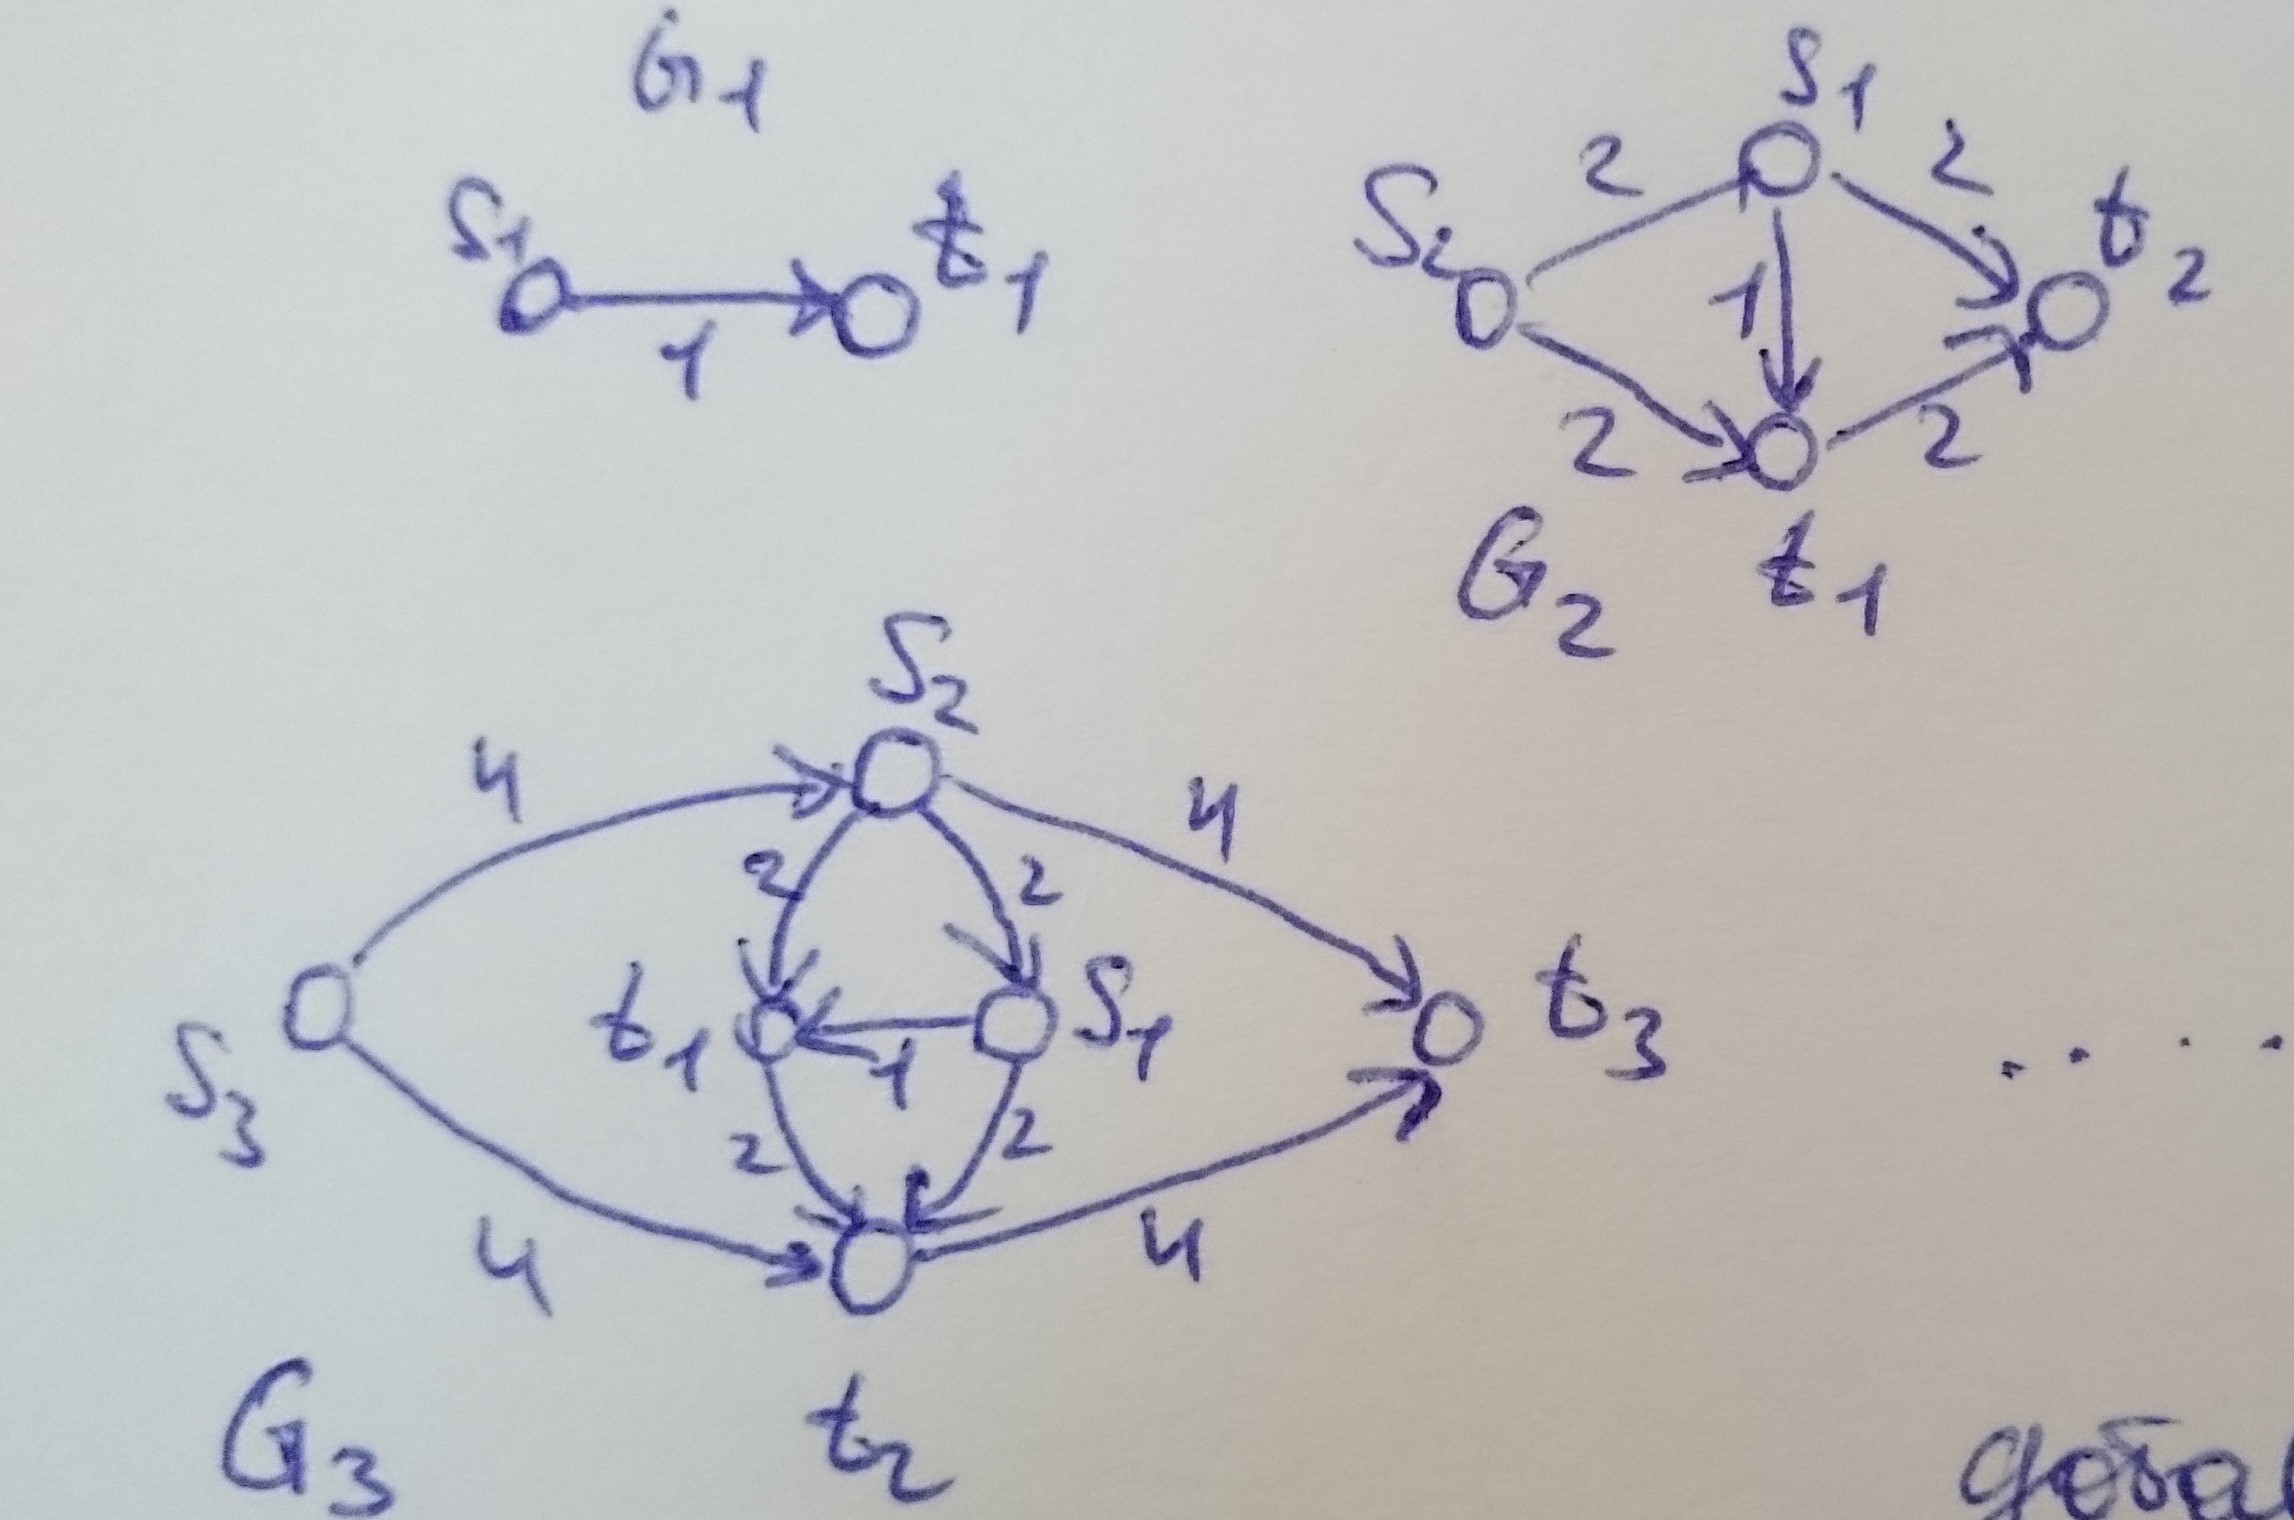
\includegraphics[scale=0.1]{ha/img/1.JPG}
	\end{center}
	То есть если $dfs$ после прохода по ребру будет заходить каждый раз в подграф меньшего размера, то за $1$ 
	итерацию поток будет увеличиваться только на единицу. И установив, вес новых рёбер как степени двойки мы 
	добьёмся экспоненциальной сложности работы алгоритма.
\end{enumerate}
	%\section*{Паросочетания}
\begin{enumerate}
	\item Докажите, что в регулярном двудольном графе есть полное паросочетание.
	
	\textbf{Решение.} 
	
	Для начала, заметим, что регулярный двудольный граф -- граф у которого степени всех вершин совпадают. Обозначим 
	это число $k$. Из этого следует, что в графе количество вершин в каждой доле совпадает(Т.к. сколько рёбер вышло 
	из первой доли, столько же должно войти во вторую долю, а раз степени всех вершин равны, то и количество 
	вершин во второй доле такое же как и в первой.).
	
	Выберем произвольное подмножество вершин одной доли. Обозначим его $T$. Из него выходит $k \cdot |T|$ рёбер.
	Эти ребра приходят в множество $N(T)$. Заметим, что $\forall T: |T|\leqslant |N(T)|$. Почему это так. 
	Предположим противное, и $|N(T)| < |T|$. Но в $N(T)$ входит $k \dot |T|$ рёбер. Но тогда, по принципу Дирихле 
	найдётся вершина, в которую входит более чем $k$ рёбер из множества $T$. Но такого быть не может -- наш 
	граф регулярный. Получили противоречие. 
	
	Заметим, что мы доказали утверждение для любого $T \subseteq X$, значит выполнены условия теоремы Холла, 
	значит в графе существует $X-$насыщенное паросочетание. Но т.к. количество вершин в обоих долях графа 
	совпадает, то это паросочетание является совершенным.
	
	\item Для заданного клетчатого поля с дырками выберите максимальное количество попарно не смежных клеток. 
	Смежными считаются клетки с общей стороной.
	
	\textbf{Решение.}
	
	Построим граф $G$. Каждой клетке будет соответствовать вершина, а ребро между двумя вершинами проведём лишь в 
	том случае, если соответствующие клетки смежные. Заметим теперь, что построенный граф $G$ является двудольным 
	- т.к. клетчатое поле может быть представлено в виде шахматной доски, но мы соединили лишь вершины разных 
	цветов, значит ребра соединяют только вершины из разных долей графа.
	
	Осталось в таком двудольном графе найти максимальное независимое множество. Воспользуемся теоремой Кёнига, 
	которая утверждает, что минимальное вершинное покрытие в двудольном графе совпадает по размеру с максимальным 
	паросочетанием. Так же нам известно, что в произвольном графе максимальное независимое множество вершин - это 
	дополнение к минимальному вершинному покрытию.
	
	Значит нам необходимо найти максимальное паросочетание, затем по этому паросочетанию построить 
	минимальное вершинное покрытие. Дополнение к минимальному вершинному покрытию образуют максимальное 
	независимое множество. Это и есть искомое подмножество.
	
	Чтобы найти минимальное вершинное покрытие можно воспользоваться теоремой Кёнига, и следующим из его 
	доказательства алгоритмом.
	
	\item Разбейте вершины ориентированного графа на циклы. Т.е. каждая вершина должна быть покрыта ровно одним 
	циклом. Либо скажите, что это невозможно.
	
	\textbf{Решение.} Допустим, что граф можно разбить на циклы, тогда рассмотрим какой-то цикл $v_1, v_2, .., 
	v_n, v_1$. В нем есть ребра $v_1 \to v_2, v_2 \to v_3, v_3 \to v_4,..., v_n \to v_1 $. Заметим, что если 
	рассмотреть двудольный граф $G$, в котором первая доля - начала ребер, а вторая доля - концы, то цикл 
	соответствует некоторому совершенному паросочетанию в таком графе. Если же циклов несколько, то 
	соответствующие двудольные графы можно слить в один большой двудольный граф. В нем будет совершенное 
	паросочетание.
	
	Теперь обратно. Пусть в двудольном графе $G = [\{v_1, v_2, ..., v_n\}, \{v'_1, v'_2, ..., v'_n\}]$ существует 
	совершенное паросочетание $M$, тогда соответствующий орграф может быть разбить на циклы. Рассмотрим 
	совершенное паросочетание. Построим цикл, покрывающий $v_1$. Пусть в $M$ вершину $v_1$ покрывает ребро $v_1 
	\to v'_j$, тогда первое ребро искомого цикла будет $v_1 \to v_j$. Второе ребро будет $v_j \to v_i$, где $v_i$ 
	это вершина, которую покрывает ребро $(v_j \to v'_i) \in M$. Продолжая, мы обязательно получим замкнутый 
	цикл, т.к. вершина $v'_1$ тоже покрыта $M$. После этого, возможно покрыты все вершины, а если нет, то 
	аналогично покроем и их.
	
	Таким образом, доказана эквивалентность существования совершенного паросочетания и возможности разбить орграф 
	на циклы, в которых каждая вершина покрыта одним циклом. Способ построения циклов описан в доказательстве 
	обратного утверждения.
	
	\item Дано $N$ различных прямых. Нужно выбрать максимальное по размеру подмножество прямых такое, что никакие 
	две прямые не параллельны, и никакие прямые не пересекаются в точке c $x = 0$.
	
	\textbf{Решение.}
	
	Заметим, что каждую прямую можно характеризовать двумя значениями: угол наклона касательной, и точкой 
	пересечения с $Oy$ (возможно отсутствующей.). Построим следующий двудольный граф $G$. В первой доли находятся 
	все значения углов наклона, во второй доле находятся все значения точек пересечения с $Oy$. Добавим в граф 
	$N$ рёбер, которые соответствуют прямым. Если в полученном двудольном графе найти максимальное паросочетание, 
	то получим ровно то, что требуется, т.к. все соответствующие прямые имеют попарно различные точки пересечения 
	с $Oy$ и углы наклона касательной. 
	 
\end{enumerate}

	\section*{Снова потоки}
\begin{enumerate}
	\item Разберитесь с пересчётом потенциалов при поиске потока.
	
	\textbf{Решение.}
	
	При после каждого запуска Дейкстры будет добавлять к потенциалу вершины минимальное расстояние от истока. Это 
	обеспечит что все расстояния будут неотрицательны, а кратчайшие пути сохранены.
	
	\item Дан массив, найдите $k$ непересекающихся возрастающих последовательностей максимальной длины за $O(kV^2)$.
	
	\textbf{Решение.}
	
	Построим сеть: каждому элементу массива $a[1..n]$ сопоставим вершину $v_i$. Рассмотрим элемент массива с 
	индексом $i$. Рассмотрим элементы с индексами $j = i + 1, i + 2, ..., n$. Если $a[i] < a[j]$, то добавим ребро 
	$v_i \to v_j$. Стоимость ребра установим в $-1$, а пропускную способность равную $1$. 
	
	Теперь добавим исток и сток. Добавим вершину $s = v_0$ - исток, соединим её со всеми $v_i, i = 1,..,n$ рёбрами 
	$v_0 \to v_i$ стоимости 0, пропускной способности $1$. Так же добавим вершину $t = v_{n + 1}$ - сток, добавим 
	ребра $v_i \to v_{n + 1}, i = 1,..,n$ стоимости $0$, пропускной способности $1$. Заметим, что теперь есть 
	проблема - через одну вершину может проходить несколько последовательностей. Чтобы это исправить, раздвоим 
	каждую вершину $v_i$ на $v_i$ и $v_i'$, и добавим ребро $v_i \to v_i'$ пропускной способности $1$. Ребра 
	входившие в $v_i$ входят в $v_i$, а ребра исходящие из $v_i$ теперь исходят только из $v_i'$.  
	
	Заметим, что все ребра в графе идут от вершин с меньшими номерами в вершины с большими номерами, значит циклов 
	отрицательного веса быть не может. Теперь, воспользовавшись результатом задачи $5$ с практики получим поток 
	минимального веса размера $k$ за $O(kn^2)$.

	
	\item Дан граф, на каждом ребре написано $2$ числа $L$ и $R$ и $c$. По каждому ребру может течь не более
	чем $R$, но не менее, чем $L$ жидкости. Найдите:
	\begin{enumerate}
		\item произвольную циркуляцию
		
		\textbf{Решение}
		
		Добавим к графу новый исток и сток $s$ и $t$. Каждое ребро заменим на три ребра. Рассмотрим ребро $(u, v)$ с ограничениями $l, r$, заменим его на ребра:
		\begin{itemize}
			\item $(s, u)$ - ребро пропускной способности $l$
			\item $(v, t)$ - ребро пропускной способности $l$
			\item $(u, v)$ - ребро пропускной способности $r - l$
		\end{itemize}
		
		Заметим, что любой поток в этой сети задаёт циркуляцию. После этого осталось лишь найти максимальный поток в полученной сети. Если удалось насытить все ребра, исходящие из истока, то требуемая циркуляция найдена.
		\item произвольный поток
		
		\textbf{Решение}
		
		Соединим исток и сток ребром пропускной способности $+\infty$, и найдём циркуляцию.
		\item максимальный поток
		
		\textbf{Решение}
		
		Заменим ребро между истоком и стоком не $+\infty$, ребром $[l, r]$, где $r = + \infty$. Осталось найти максимальное $l$ при которой существует циркуляция. Сделаем это с помощью линейного поиска.
		\item поток минимальной стоимости.
		
	\end{enumerate}
	
	\item Есть $k$ одинаковых автоматов и $n$ заданий. Про каждое задание известно, во сколько его нужно начать 
	делать, во сколько закончить, а также его стоимость. Каждый автомат может выполнять только одно задание в 
	каждый момент времени. Нужно выполнить задания максимальной суммарной стоимости. $O(kn \log n)$.
	
	\textbf{Решение.}
	
	Все задания задают два момента времени -- начало и конец задания, а также стоимости $c_i$. Каждому такому 
	моменту времени зададим вершину. Получится $2n$ вершин. Вершину соединим ребром с вершиной - соответствующим 
	следующему моменту времени (предварительно времена нужно отсортировать). Вес такого ребра сделаем равным $0$, 
	а пропускную способность $+\infty$. Добавили $2n - 1 = O(n)$ ребер. Теперь добавим ещё $n$ ребер. Для каждого 
	задания соединим вершину начала задания - с вершиной концом задания ребром пропускной способности $1$, 
	стоимости $-c_i$. Теперь осталось найти поток величины $k$ с минимальной стоимостью между вершиной начального 
	момента времени, и конечного момента времени. Т.к. граф ациклический - все ребра идут от меньшего момента 
	времени к большему, то отрицательных циклов быть не может. Значит, за $O(k)$ запусков алгоритм Дейкстры мы 
	сможем найти требуемый поток. 
	
	Сложность: $O(n\log n) + O(n) + O(kE\log V)$. Заметив, что $V = O(n), E = O(n)$. Получим итоговую оценку $O(kn\log n)$.
	
\end{enumerate}

\end{document}

